\subsection{Proposed Research}
We propose to investigate several runtime optimization techniques to make~\systemname~suitable for wearable devices without changing the off-the-shelf hardware by  minimizing the authentication latency and energy consumption. Please note that we could choose to offload computation to the device-paired smartphone to conserve cycles/energy on the wearable device, but \emph{we will not pursue this route in this proposal.} Instead, we focus on \emph{direct authentication} where wearable devices are not dependent upon smartphones or other more powerful devices for authentication, which we believe is more secure and convenient.

As discussed in Sec~\ref{sec:learning}, a~\systemname~authentication session consists of the following steps: (1) collecting test data, (2) extracting features from the test data, and (3) classifying the test data. Among these three steps, steps (2) and (3) usually consume more processing cycles/energy. In this project, we focus on optimizing these two steps. Before we present the proposed optimization techniques, we note that the first thing we need to is to carefully select features and classifiers in~\systemname~from the set of features discussed in Sec~\ref{sec:features}. We already know that using too many features may lead to noises and classification errors~\cite{***}, but on wearable devices, this is even more catastrophic as it likely leads to quick device shutdown. As a result, we need to pay extra attention to what features we use and which classifier we adopt on the device. In the project, we will carefully measure the power consumption, processing delay, and classification accuracy of different combinations of features and classifiers, and then choose accordingly.

\begin{wrapfigure}{r}{3.0in}\centering
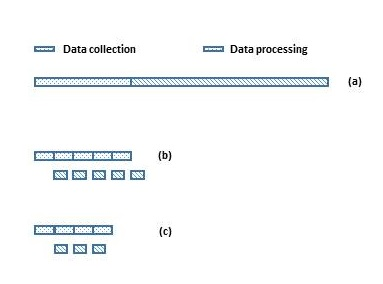
\includegraphics[width=0.75\linewidth]{../figure/pipeline.jpg} \\
\caption{\label{fig:pipeline} The benefit of pipelined authentication: (a) shows the original latency to collect and process a 10-second sample (numbers taken from Figure~\ref{tab:glass}, (b) shows the much reduced latency by breaking the 10-second signal to five 2-second chunks and pipeline the collection and processing procedures, and (c) shows that the delay can be further reduced if using a portion of the signal can correctly infer the classification result.}
\vspace{-6pt}
\end{wrapfigure}
\vspace{4pt}\textbf{Pipelined Authentication:} An important parameter for~\systemname~is the sample duration $T$. So far, we assume that the system first collects $ACC$ sample for $T$ seconds, and then processes the sample (i.e., feature extraction and classification) to obtain the classification result. The value of $T$ directly impacts the total authentication latency; larger $T$ values lead to longer authentication latencies.  From our preliminary investigation, we further take note that the processing delay increases more than linearly with sample duration -- e.g., processing a 2-second sample takes 1.29 seconds, while processing a 10-second sample takes 20.48 seconds (according to Figure~\ref{tab:glass}). As a result, we would like to have lowest possible $T$ values. On the other hand, however, having a too small $T$ value may lead to inferior authentication accuracies. What further complicates the problem is that we find that it is impossible to find the uniformly optimal $T$ value for different users. Thus optimizing this important parameter across different users becomes a serious challenge.

In this project, we propose to address this challenge by adopting the well-known pipeling technique, which is motivated by the characteristics of~\systemname. Suppose the original signal duration is $T$, and we have $T=nt$ with $n$ being an integer and $t<2$ seconds. Let us assume that the processing delay is less than $t$ when the sample duration $t$ is less than 2 seconds.  Then we can explore the following pipelining method. In the first $t$-second window, the system collects the $ACC$ sample for $t$ seconds. In any subsequent $t$-second window, the system continues to collect the $ACC$ sample for $t$ seconds, and at the same time, processes the portion of the sample collected in the previous window. We refer to this method as \emph{pipelined authentication}.


The proposed pipelined authentication can reduce the overall authentication latency in several ways. First, we overlap data collection and data processing to reduce the overall delay. Second, since processing shorter samples incurs less (than linear) latencies, by breaking a sample into smaller chunks can reduce the total latency. For example, using the numbers presented in Figure~\ref{tab:glass}, we find that processing one 10-second sample takes much longer time than processing one 6-second, one 2-second, and two 1-second samples. Third, now we can conduct what we call ``early classification'' -- maybe using a portion of the sample can already reveal the classification result -- and then we don't need to collect/process the entire sample. That is, we can dynamically determine the shortest sample duration we need. Combing these two factors, we can achieve much reduced authentication latency (i.e., shorter data collection and shorter processing delays). Figure~\ref{fig:pipeline} illustrates the benefit of the proposed pipelined authentication scheme.

Finally, we note that in order to take the full advantage of pipelined authentication, we need to choose appropriate features whose performance is not highly dependent on the sample duration. For example, ***.


\vspace{4pt}\textbf{Authentication with Fewer Samples:} Another optimization we will explore is authenticating users with fewer samples. We can attempt to reduce the number of samples in several ways. First, we can minimize the number of samples for the legitimate user in the training set. It is thus a tricky question to determine how many and which samples should be used. In this project, we will explore only using the ``representative'' samples -- i.e., those that are the most similar to the rest of the user's samples. In this way, the computation/energy consumption in the authentication session can be greatly reduced.

Another optimization technique we can adopt is to dynamically adjust the sampling rate in the test phase. A lower sampling rate leads to fewer data points in a sample, thus shorter collection and processing latencies. In this project, we will explore dynamically adjusting the sampling rate based upon the temperature of the device. Namely, if we notice the device is becoming heated, then we should reduce the sampling rate. In the project, we will carefully quantify the interaction between the device temperate and the sampling rate.

